\section{Systemdenken \& Systemdynamik}
\subsection{Einführung}
\begin{multicols}{2}
	\subsubsection{Kausales Modell}
	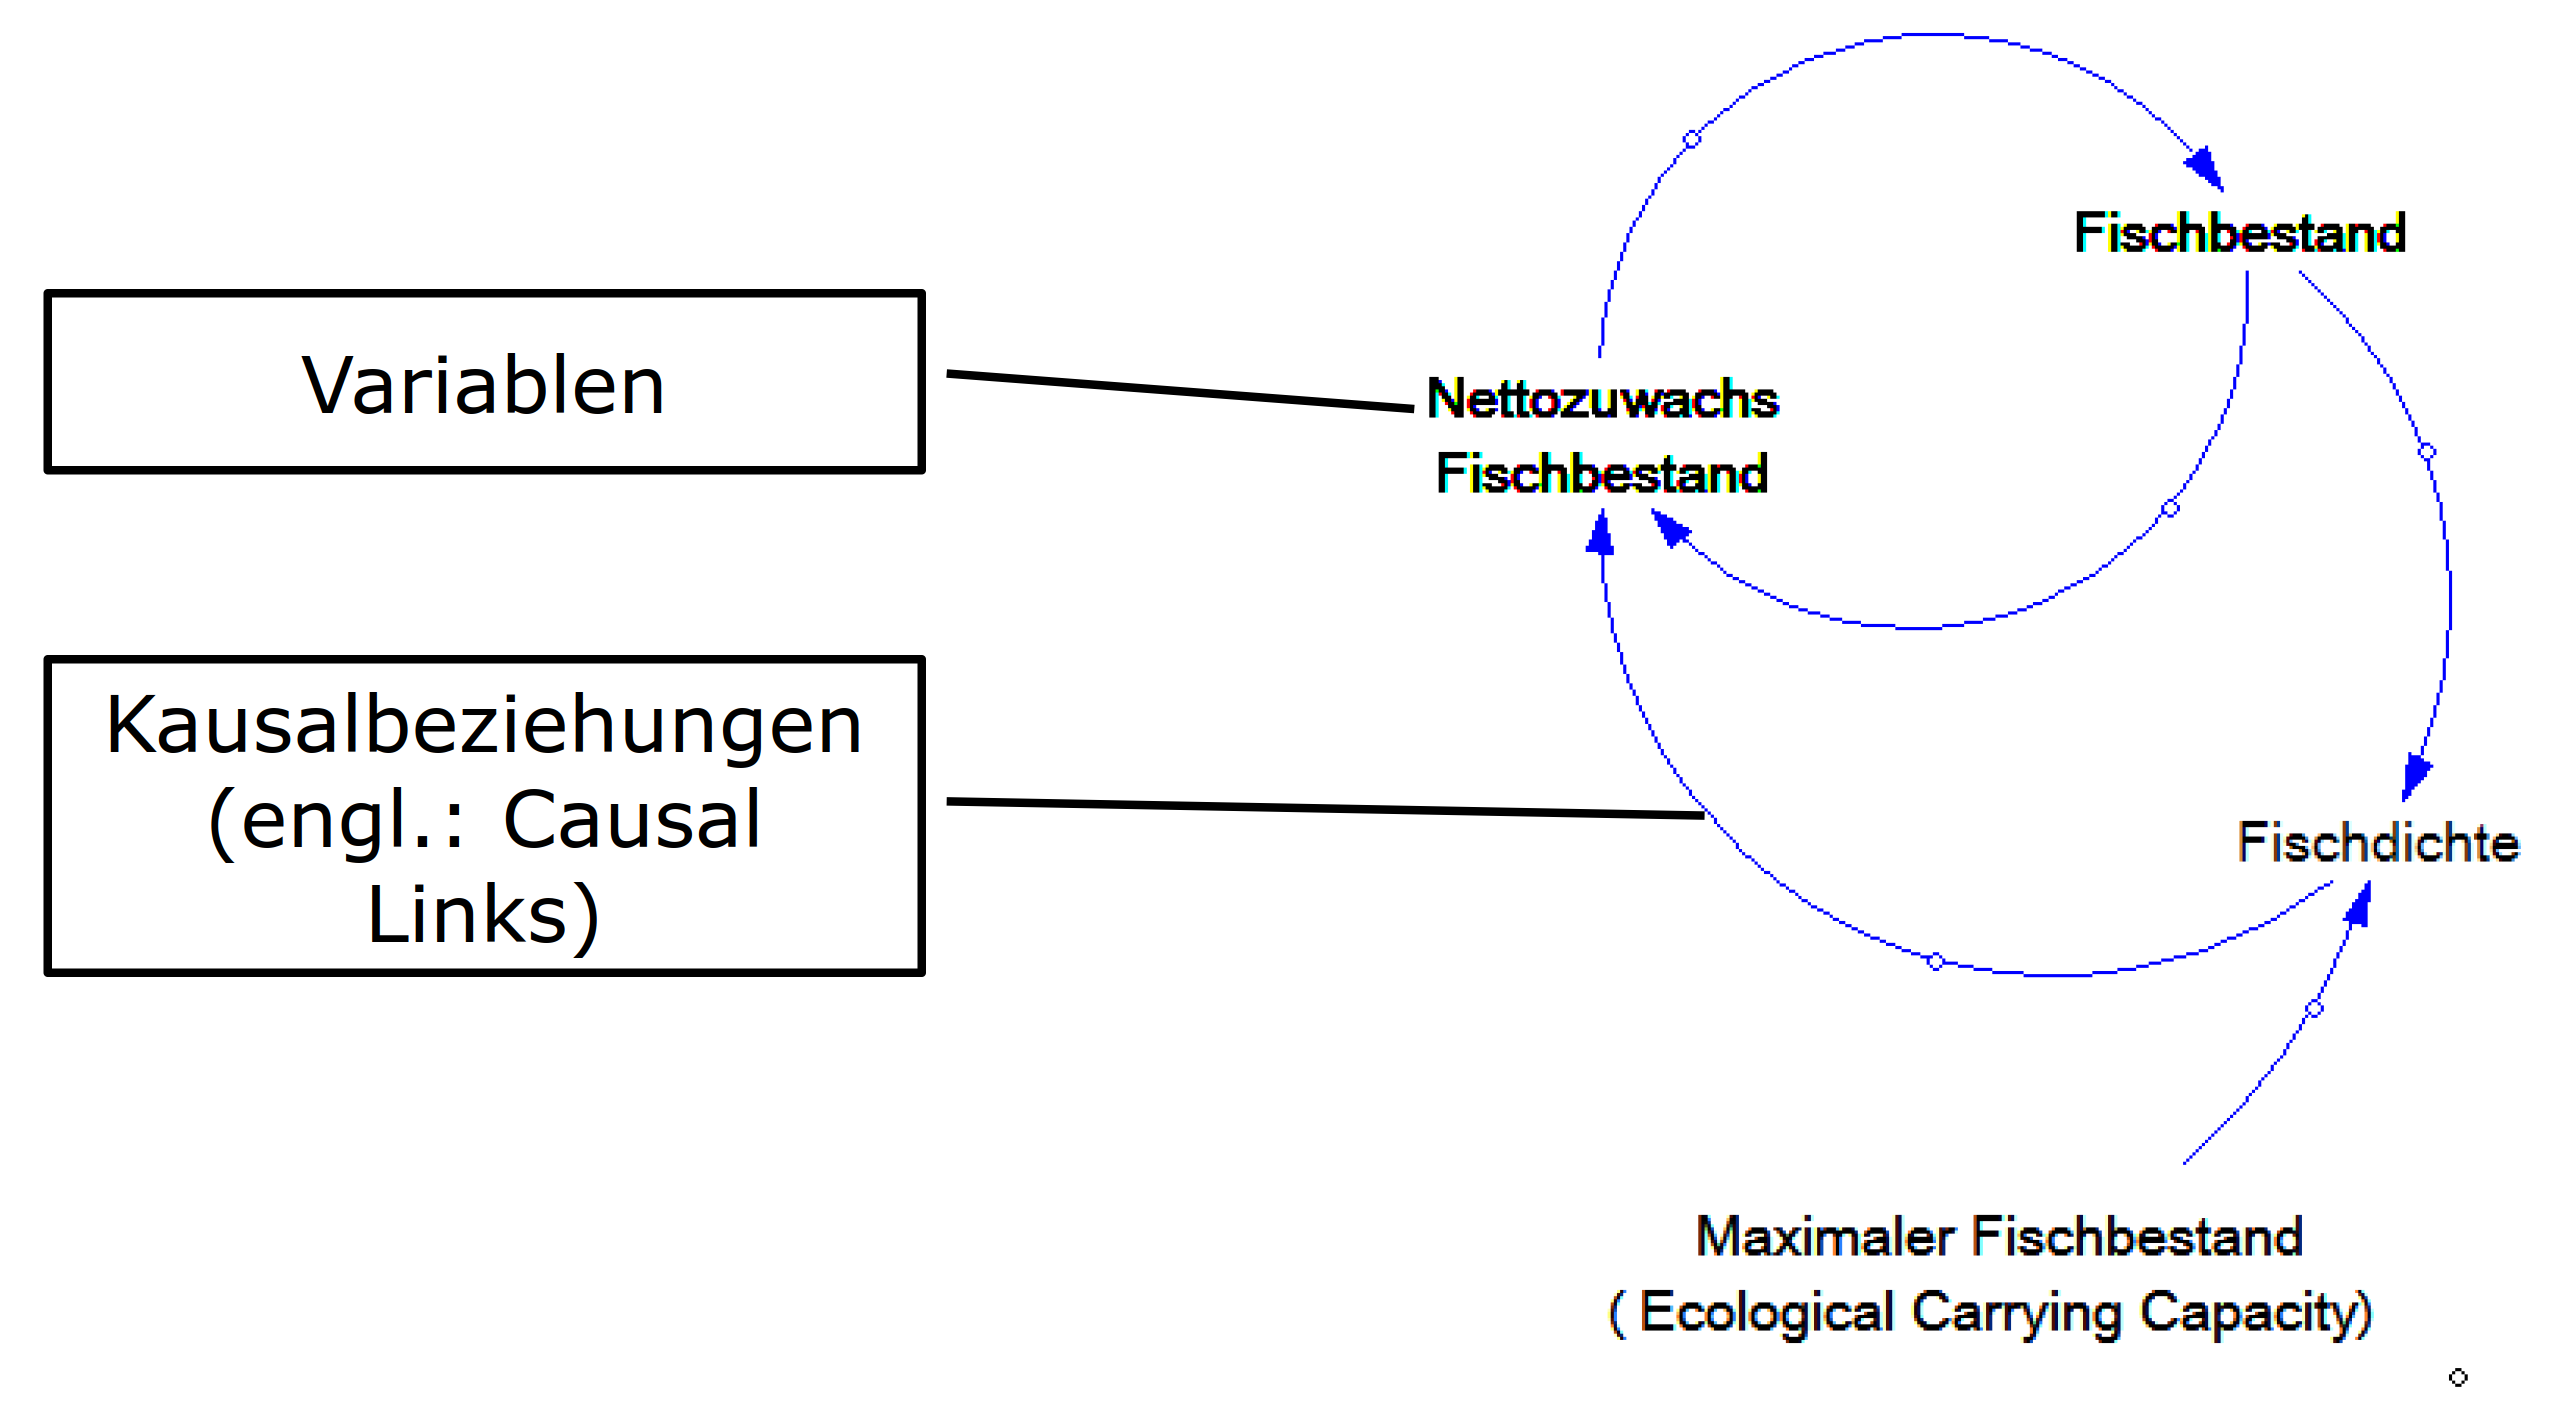
\includegraphics[width=0.5\textwidth]{pictures/kausales_modell}

	\subsubsection{Polarität einer Kausalbeziehung}
	\textbf{Positive Polarität:} Steigt (fällt) Ursache, dann steigt (fällt) Wirkung \\
	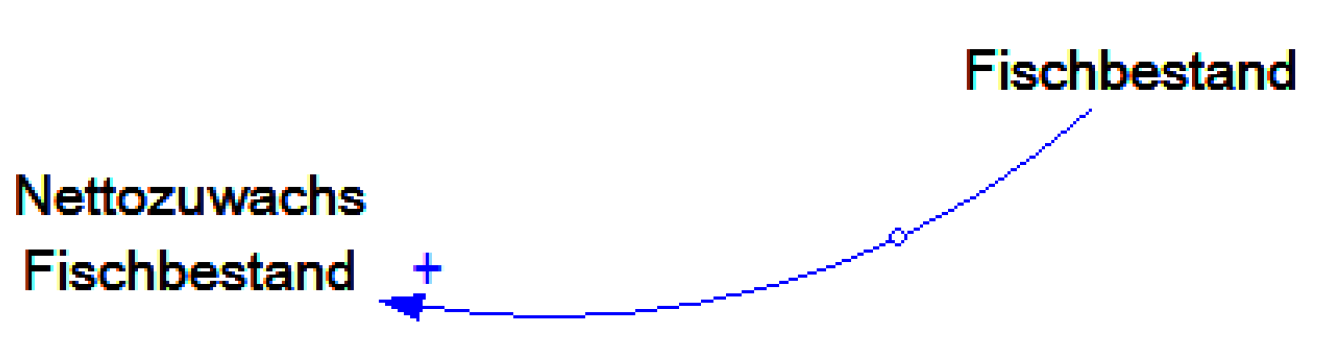
\includegraphics[width=0.35\textwidth]{pictures/positive_polaritaet}\\
	\textbf{Negative Polarität:} Steigt (fällt) Ursache, dann fällt (steigt) Wirkung \\
	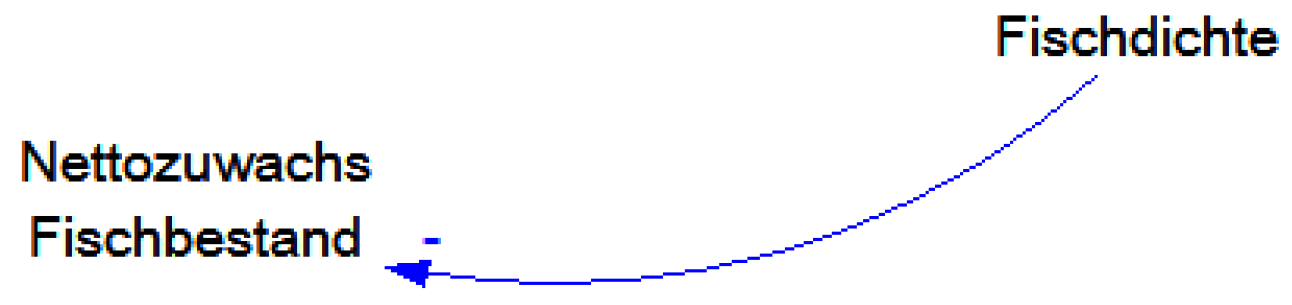
\includegraphics[width=0.35\textwidth]{pictures/negative_polaritaet}
\end{multicols}

\begin{multicols}{3}
	\subsubsection{Rückkopplung}
	Gerichteter Kreis von Kausalbeziehungen. \\
	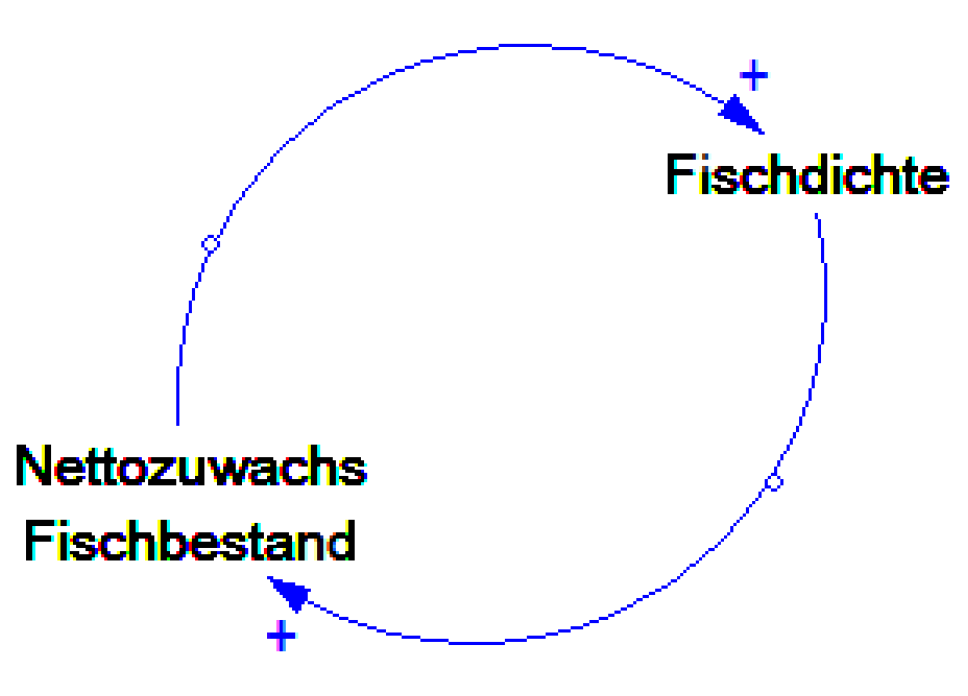
\includegraphics[width=0.25\textwidth]{pictures/rueckkopplung} \\
	
	\subsubsection{Selbstverstärkender Loop}
	Die Rückkoppelung verstärkt einen anfänglichen Effekt. \\
	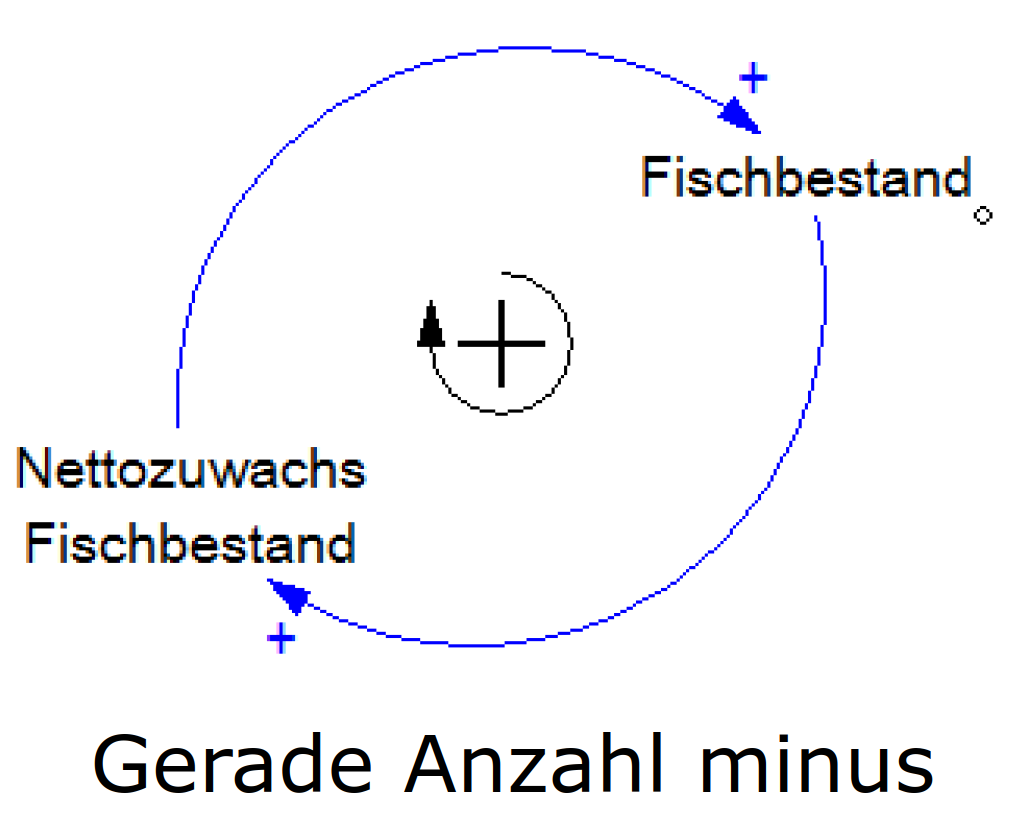
\includegraphics[width=0.25\textwidth]{pictures/selbstverstaerkender_loop}
	
	\subsubsection{Ausgleichender Loop}
	Die Rückkoppelung wirkt	einem anfänglichen Effekt entgegen.\\
	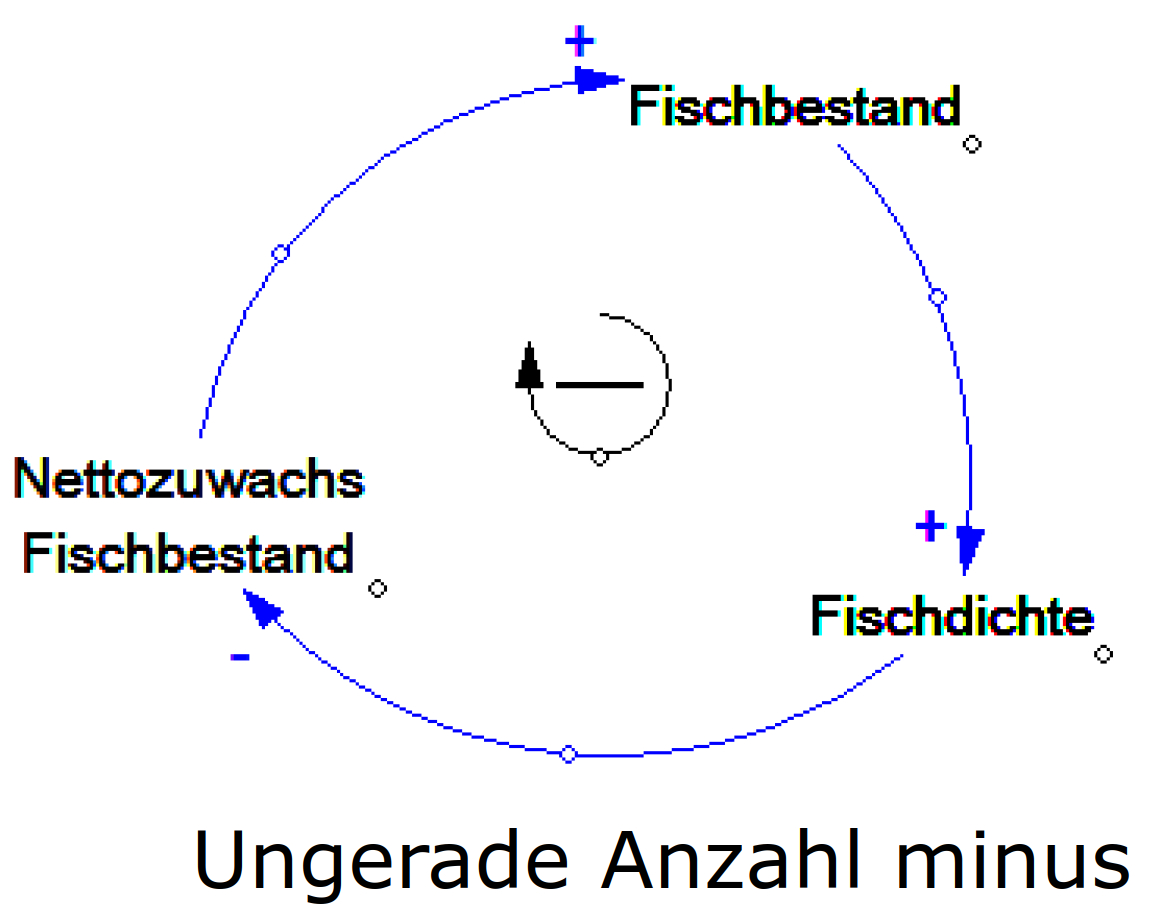
\includegraphics[width=0.25\textwidth]{pictures/ausgleichender_loop}
\end{multicols}	

\begin{multicols}{2}
	\subsubsection{Stock-and-Flow Diagramm}
	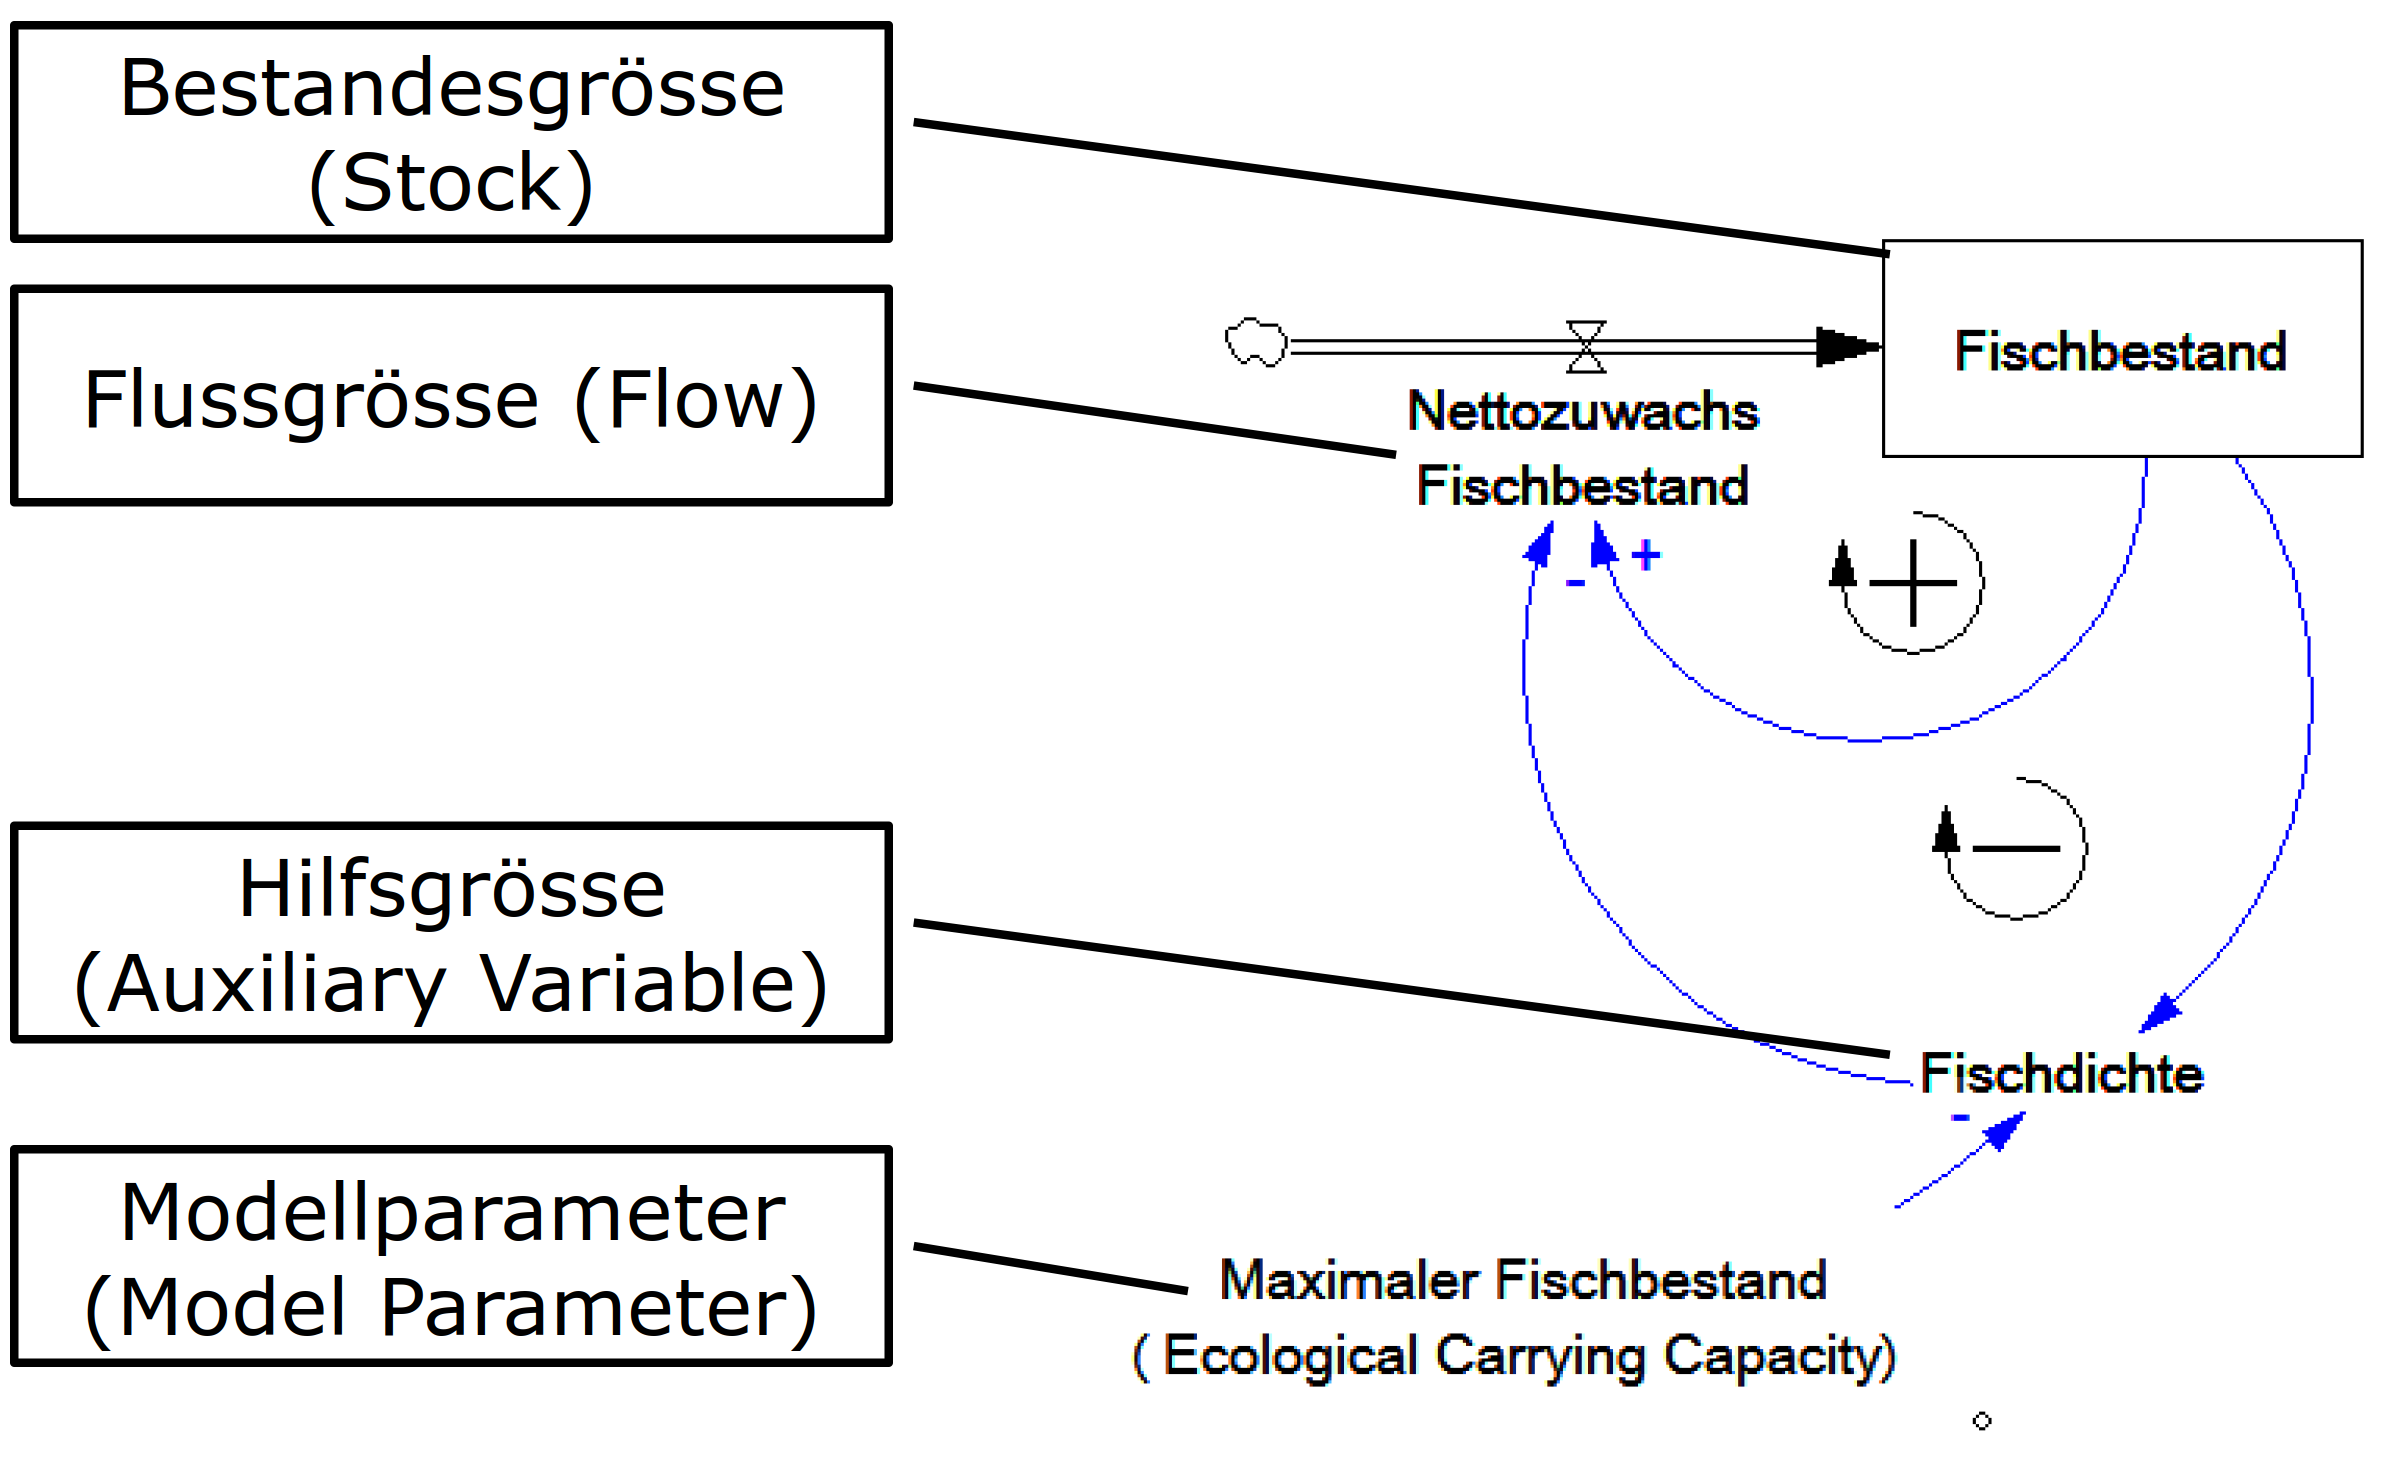
\includegraphics[width=0.5\textwidth]{pictures/stock_and_flow_diagramm}
	
	\subsubsection{Systemdynamisches Simulationsmodell}
	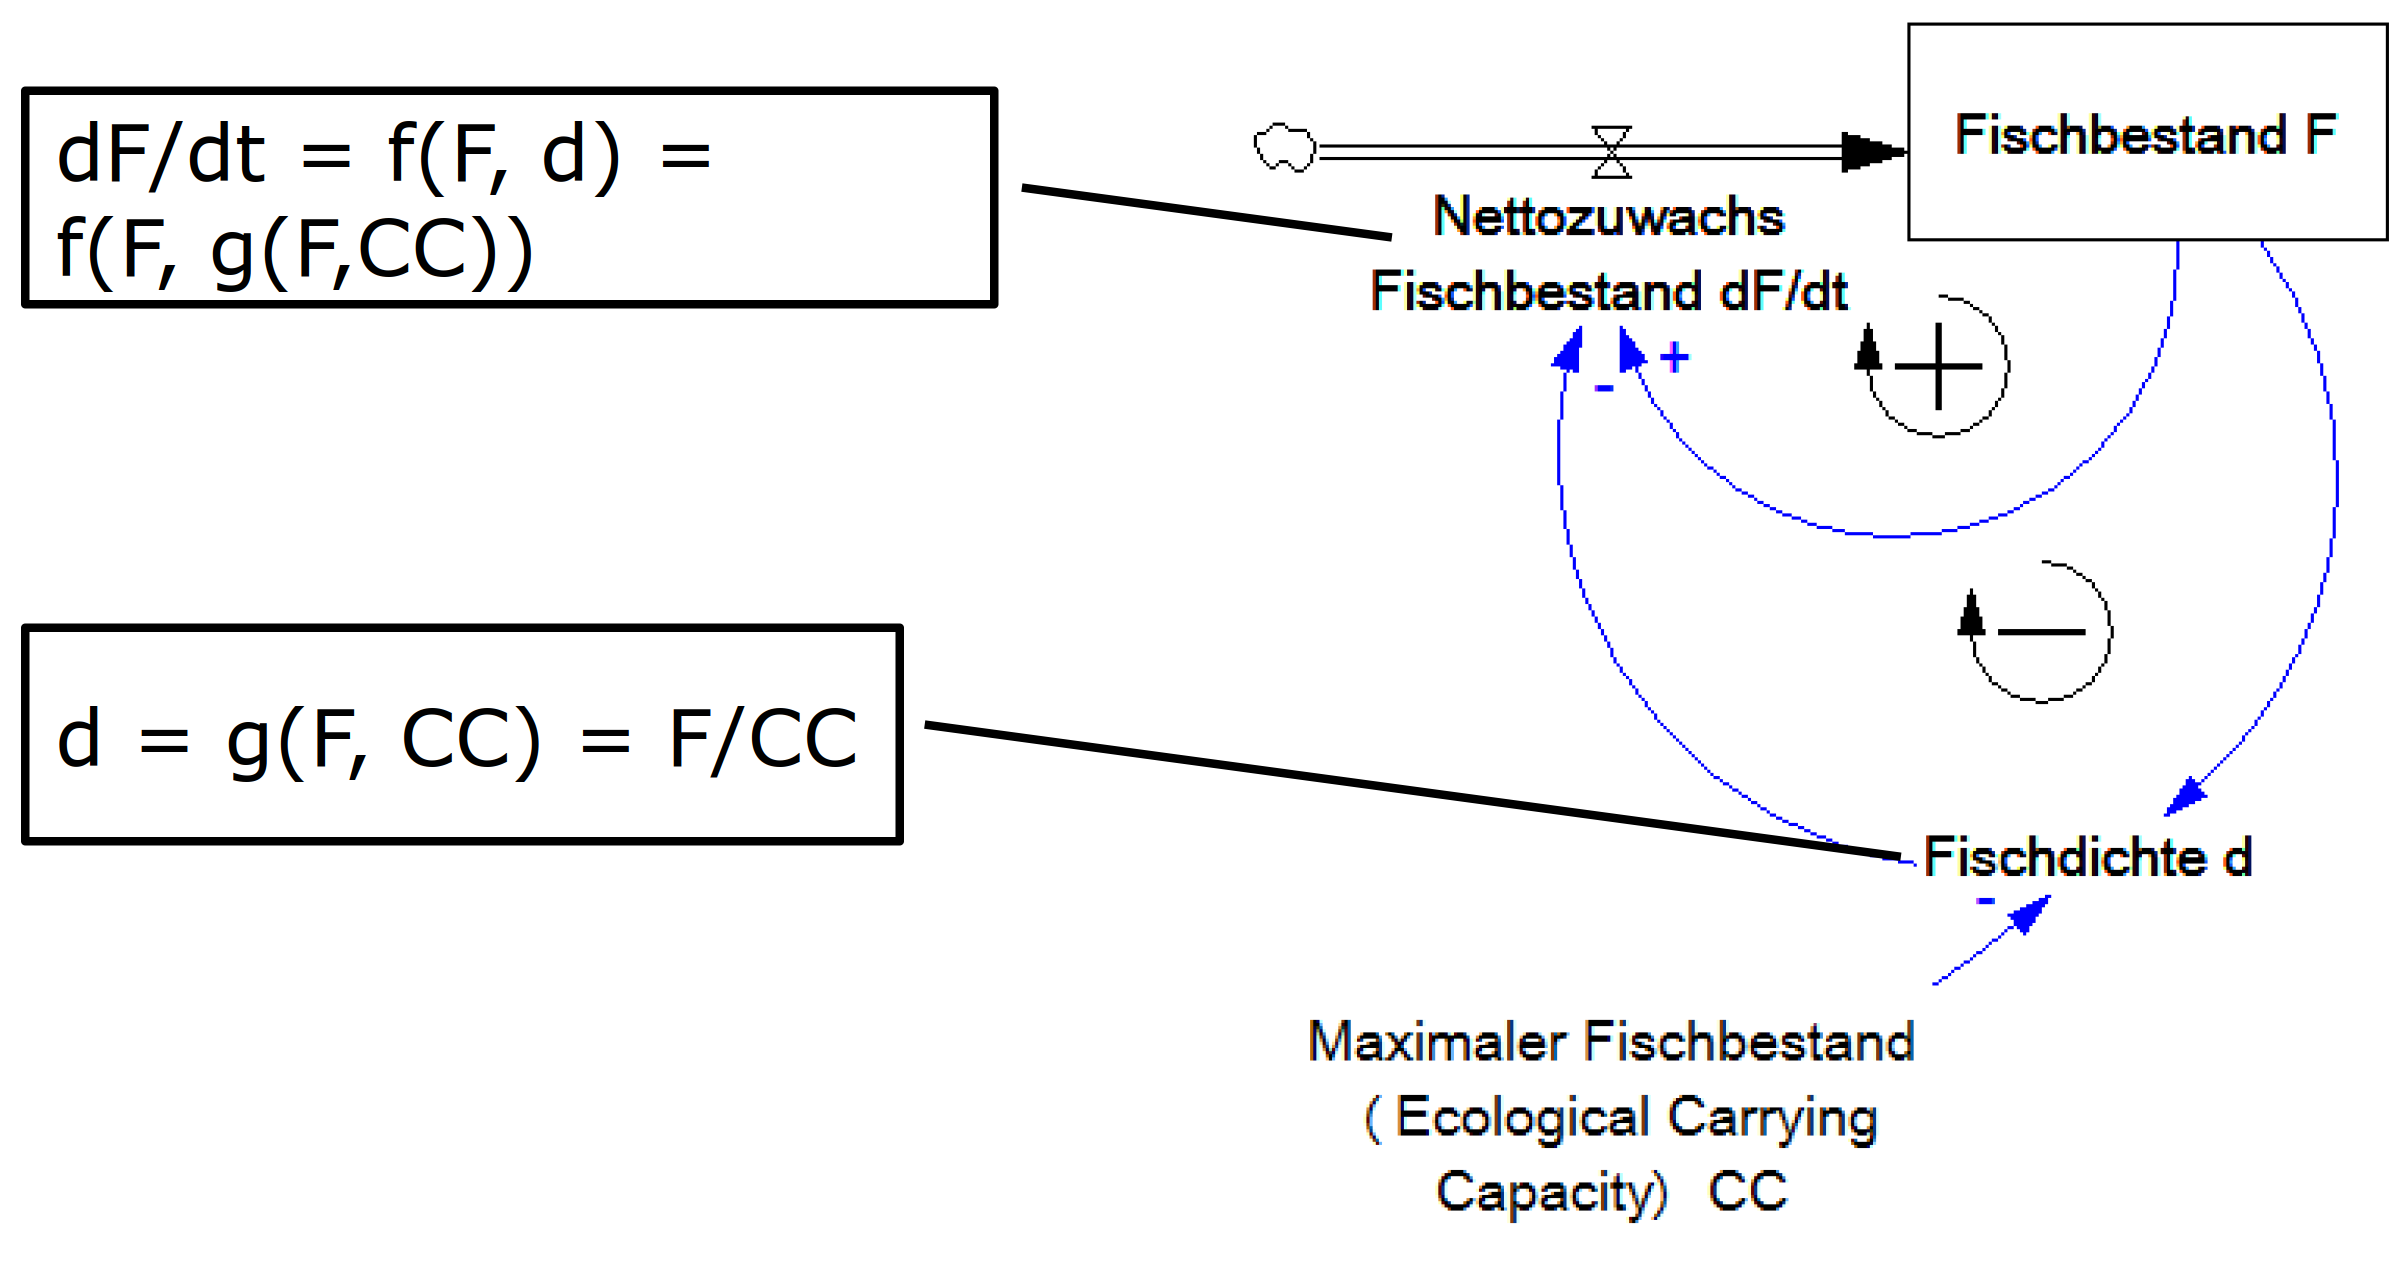
\includegraphics[width=0.5\textwidth]{pictures/systemdynamisches_simulationsmodell}
\end{multicols}	

\subsection{Grundideen}
